\nxsection{Les Localisations}
\index{localisation}

Une localisation repr\'esente une boutique ou un d\'ep\^ot
de l'entreprise utilisant \yeren.

Les informations sur une localisation permettent de
se connecter \`a la base de donn\'ees de la boutique
ou du d\'ep\^ot qu'elle repr\'esente.

\nxsubsection{Afficher les d\'etails d'une localisation}
\index{afficher les d\'etails d'une localisation}
\index{d\'etails d'une localisation}

La figure~\ref{fig:admin-localisations-afficher-details} illustre
l'interface graphique de \yeren qui affiche les d\'etails
d'une localisation.\\

\begin{figure}[!htpb]
	\centering
	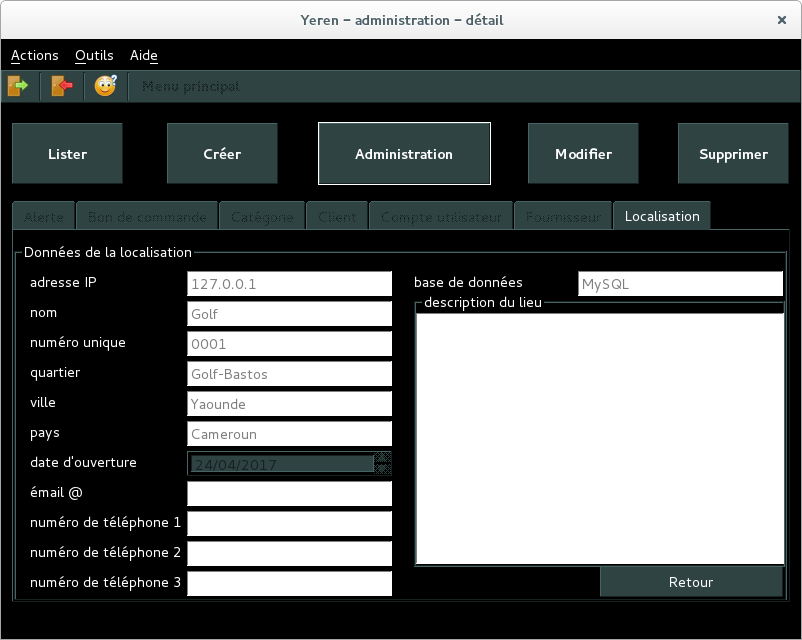
\includegraphics[scale=0.45]{images/localisation-afficher-details.png}
	\caption{L'interface graphique pour afficher les d\'etails
			d'une localisation.}
	\label{fig:admin-localisations-afficher-details}
\end{figure}

\procparagraph{Proc\'edure pour afficher les d\'etails d'une localisation}
\begin{enumerate}[1)]
	\item \`A partir de l'interface graphique de l'acceuil de
		l'administration (voir figure~\ref{fig:fenetre-administrateur}),
		on clique sur l'onglet intitul\'e \textbf{op\'erations}. 
		
	\item Choisir '\textbf{lister}' dans le '\emph{combo box
		op\'erations}'.
		
	\item Choisir '\textbf{une localisation}' dans le '\emph{combo box
		sujets}'. Vous \^etes automatiquement conduit \`a la fen\^etre
		illustr\'ee par la figure~\ref{fig:admin-localisations-lister}.
		
	\item S\'electionner la localisation dont vous souhaitez afficher
		les d\'etails dans la liste des localisations affich\'ee.
		
	\item Cliquer sur le bouton \bouton{Afficher}. Les d\'etails
		sur la localisation choisie sont affich\'es dans
		une nouvelle fen\^etre.
\end{enumerate}

%%%%%%%%%%%%%%%%%%%%%%%%%%%%%%%%%%%%%%%%%%%%%%%%%%%%%%%%%%%%%%%%%%%%%%%%%%%%%%%%%

\nxsubsection{Cr\'eer une localisation}
\index{cr\'eer une localisation}

La figure~\ref{fig:admin-localisations-creer} illustre
l'interface graphique de \yeren pour cr\'eer une localisation.\\

\begin{figure}[!htpb]
	\centering
	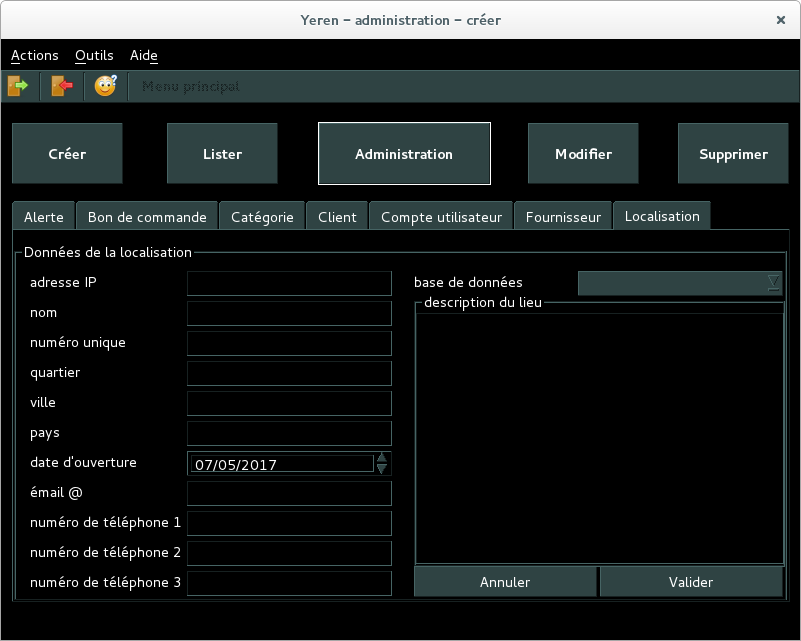
\includegraphics[scale=0.45]{images/localisation-creer.png}
	\caption{L'interface graphique pour cr\'eer une localisation.}
	\label{fig:admin-localisations-creer}
\end{figure}

\procparagraph{Proc\'edure pour cr\'eer une localisation}
\begin{enumerate}[1)]
	\item \`A partir de l'interface graphique de l'acceuil de
		l'administration (voir figure~\ref{fig:fenetre-administrateur}),
		on clique sur l'onglet intitul\'e \textbf{op\'erations}. 
		
	\item Choisir '\textbf{cr\'eer}' dans le '\emph{combo box
		op\'erations}'.
		
	\item Choisir '\textbf{une localisation}' dans
		le '\emph{combo box objets}'. Vous \^etes automatiquement
		conduit \`a la fen\^etre illustr\'ee par la
		figure~\ref{fig:admin-localisations-creer}.
		
	\item Saisissez les informations requises dans les champs
		de texte suivants:
		\begin{enumerate}[1)]
			\item adresse IP 
			\item nom \obligatoire
			\item num\'ero unique 
			\item quartier
			\item ville
			\item province / \'etat
			\item pays
			\item bo\^ite postale
			\item date d'ouverture
			\item \'email@
			\item num\'ero de t\'el\'ephone 1
			\item num\'ero de t\'el\'ephone 2	
			\item base de donn\'ees					
			\item description du lieu.\\
		\end{enumerate}
		
		Si vous avez entr\'e une adresse IP pour cette 
		localisation, vous devez choisir le type de base de
		donn\'ees utilis\'e dans cette localisation. Pour
		l'instant, \yeren ne fonctionne qu'avec \emphbf{MySQL}.\\
		
		La section~\ref{sec:yeren-sgbd} dans
		l'annexe~\ref{chap:environement-logiciel-requis}
		(L'Environnement Logiciel) contient plus d'information
		aux sujets des bases de donn\'ees dans \yeren.
		
	\item Cliquer sur le bouton \bouton{Valider} pour
		valider votre travail.	
\end{enumerate}

%%%%%%%%%%%%%%%%%%%%%%%%%%%%%%%%%%%%%%%%%%%%%%%%%%%%%%%%%%%%%%%%%%%%%%%%%%%%%%%%%

\newpage
\nxsubsection{Lister les localisations}
\index{lister les localisations}

La figure~\ref{fig:admin-localisations-lister} illustre
l'interface graphique de \yeren qui liste les localisations.\\

\begin{figure}[!htpb]
	\centering
	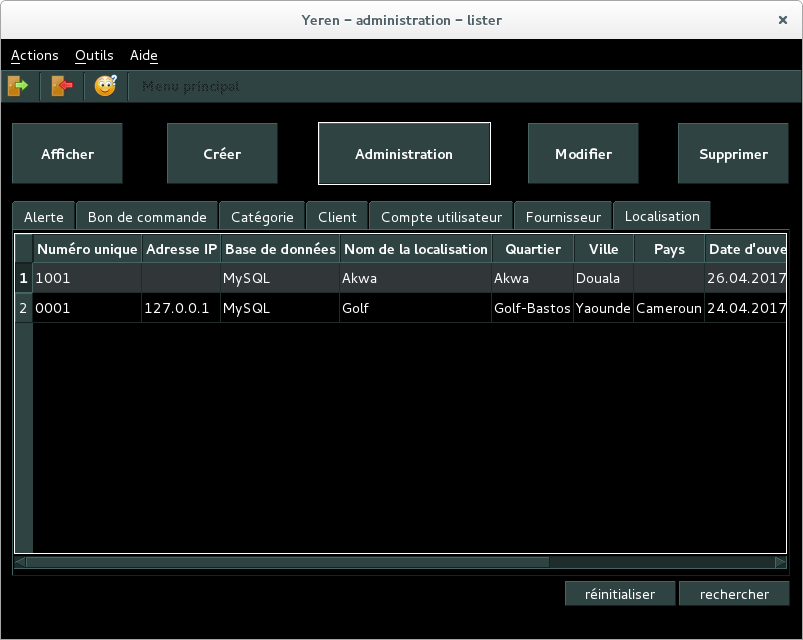
\includegraphics[scale=0.45]{images/localisation-lister.png}
	\caption{L'interface graphique pour cr\'eer une localisation.}
	\label{fig:admin-localisations-lister}
\end{figure}

\procparagraph{Proc\'edure pour lister les localisations}
\begin{enumerate}[1)]
	\item \`A partir de l'interface graphique de l'acceuil de
		l'administration (voir figure~\ref{fig:fenetre-administrateur}),
		on clique sur l'onglet intitul\'e \textbf{op\'erations}. 
		
	\item Choisir '\textbf{lister}' dans le '\emph{combo box
		op\'erations}'.
		
	\item Choisir '\textbf{une localisation}' dans le
		'\emph{combo box objets}'. Vous \^etes automatiquement
		conduit \`a la fen\^etre qui liste localisations
		(figure~\ref{fig:admin-localisations-lister}).
\end{enumerate}

%%%%%%%%%%%%%%%%%%%%%%%%%%%%%%%%%%%%%%%%%%%%%%%%%%%%%%%%%%%%%%%%%%%%%%%%%%%%%%%%%

\newpage
\nxsubsection{Modifier les d\'etails d'une localisation}
\index{modifier les d\'etails d'une localisation}

La figure~\ref{fig:admin-localisations-modifier} illustre
l'interface graphique de \yeren pour modifier les d\'etails
d'une localisation.\\

\begin{figure}[!htpb]
	\centering
	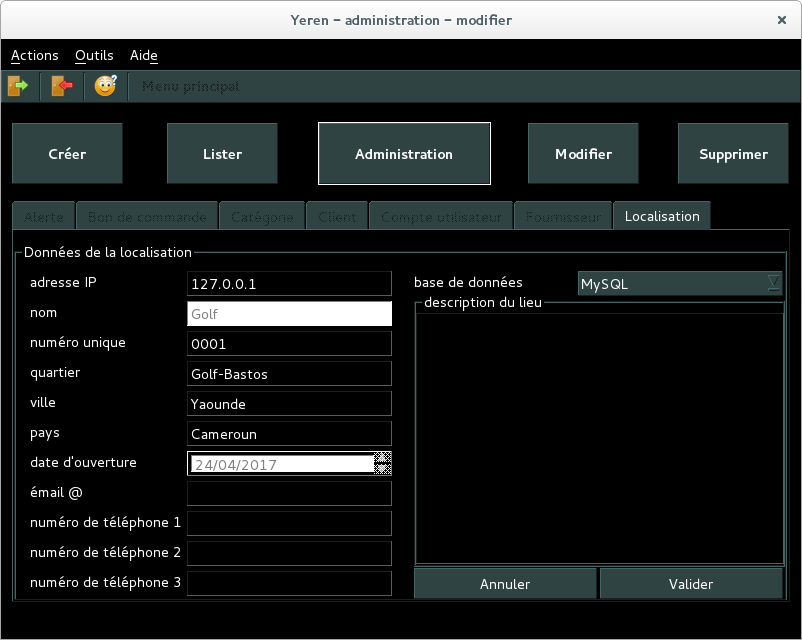
\includegraphics[scale=0.45]{images/localisation-modifier.png}
	\caption{L'interface graphique pour modifier les d\'etails
			d'une localisation.}
	\label{fig:admin-localisations-modifier}
\end{figure}

\procparagraph{Proc\'edure pour modifier les d\'etails d'une localisation}
\begin{enumerate}[1)]
	\item \`A partir de l'interface graphique de l'acceuil de
		l'administration (voir figure~\ref{fig:fenetre-administrateur}),
		on clique sur l'onglet intitul\'e \textbf{op\'erations}. 
		
	\item Choisir '\textbf{lister}' dans le '\emph{combo box
		op\'erations}'.
		
	\item Choisir '\textbf{une localisation}' dans
		le '\emph{combo box objets}'. Vous \^etes automatiquement
		conduit \`a la fen\^etre illustr\'ee par la
		figure~\ref{fig:admin-localisations-lister}.
		
	\item S\'electionner la localisation dont vous souhaitez
		modifier les d\'etails dans la liste des localisations
		affich\'ee.
		
	\item Cliquer sur le bouton \bouton{Modifier}. Les d\'etails
		de la localisation sont affich\'es dans une nouvelle
		fen\^etre.
		
	\item Faites les modifications que vous souhaitez.
		
	\item Cliquer sur le bouton \bouton{valider} pour valider
		les modifications faites.
\end{enumerate}

%%%%%%%%%%%%%%%%%%%%%%%%%%%%%%%%%%%%%%%%%%%%%%%%%%%%%%%%%%%%%%%%%%%%%%%%%%%%%%%%%

%\newpage
\nxsubsection{Supprimer une localisation}
\index{supprimer une localisation}

La figure~\ref{fig:admin-localisations-supprimer} illustre
l'interface graphique de \yeren pour supprimer une localisation.\\

\begin{figure}[!htpb]
	\centering
	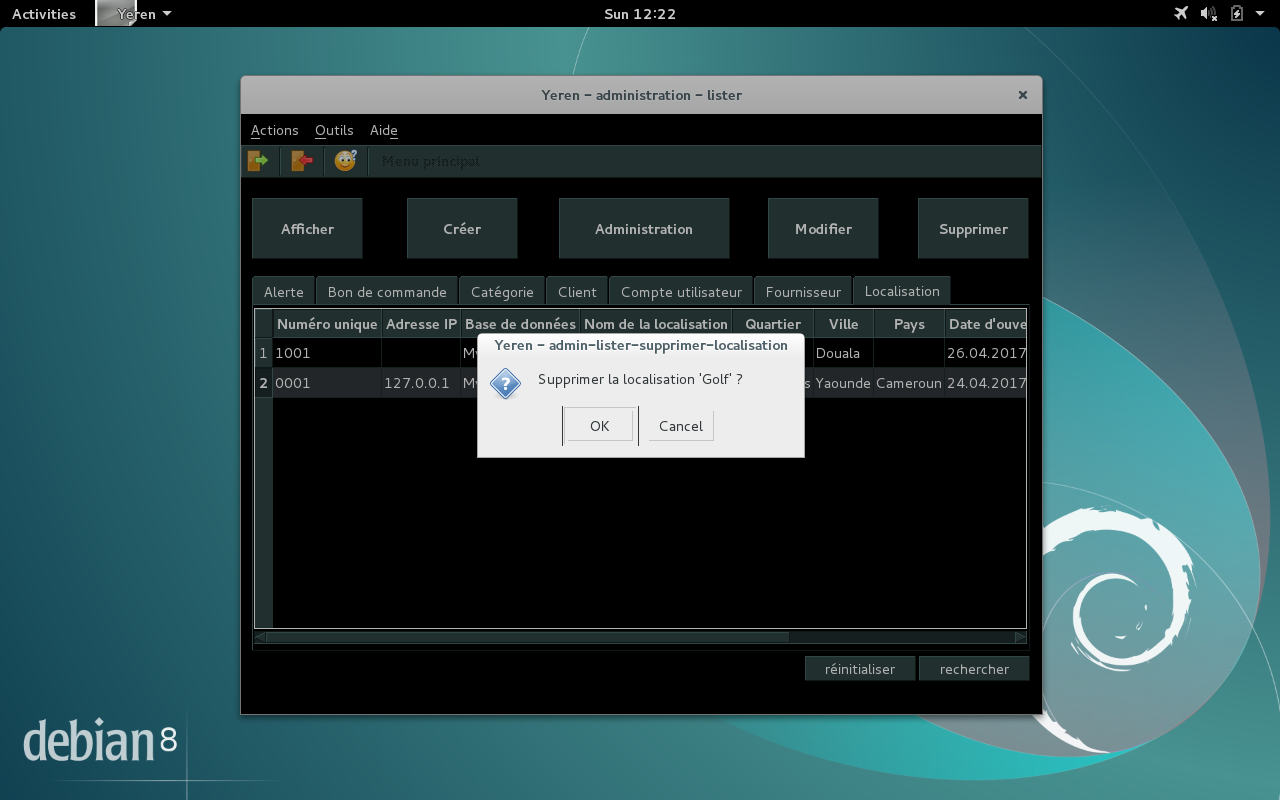
\includegraphics[scale=0.35]{images/localisation-supprimer.png}
	\caption{L'interface graphique pour supprimer une localisation.}
	\label{fig:admin-localisations-supprimer}
\end{figure}

\procparagraph{Proc\'edure pour supprimer une localisation}
\begin{enumerate}[1)]
	\item \`A partir de l'interface graphique de l'acceuil de
		l'administration (voir figure~\ref{fig:fenetre-administrateur}),
		on clique sur l'onglet intitul\'e \textbf{op\'erations}. 
		
	\item Choisir '\textbf{supprimer}' dans le '\emph{combo box
		op\'erations}'.
		
	\item Choisir '\textbf{une localisation}' dans le '\emph{combo box
		sujets}'. Vous \^etes automatiquement conduit \`a la fen\^etre
		illustr\'ee par la figure~\ref{fig:admin-localisations-lister}.
		
	\item S\'electionner la localisation \`a supprimer dans la liste
		des localisations affich\'ee.
		
	\item Cliquer sur le bouton \bouton{Supprimer}. La question
		est ensuite pos\'ee si vous confirmer votre choix.
		Cliquer sur le \bouton{OK} pour confirmer votre choix.
\end{enumerate}
